Artificial intelligence (AI) is another field of computing which strains classical computers, so building systems that can achieve anything resembling intelligence requires very powerful computers~\cite{to-build-a-brain-6247562}. In 1997, IBM's Deep Blue computer won a game of chess to human master Garry Kasparov, but to do this, it relied on 480 specialized chess chips that performed massively parallel game moves searches~\cite{deep-blue-Campbell200257}. Although it was not the first attempt at hardware-based AI~\cite{indiveri2011frontiers}, it was probably the first time a general audience got to know that a computer could beat a human being on cognitive tasks. 

In 2013, a neural simulation consisting of 1.73 billion neurons and 10.4 trillion synapses was performed. The largest simulation of its time used the K supercomputer, utilizing 82,944 SPARC64 VIIIfx processors. The software simulated the network for 40 minutes, which was equivalent of the activity of 1\% of the human brain for 1$s$.

This great achievement may be dwarfed by the fact that humans can do much more than play chess and Deep Blue was nowhere near ready to do the laundry or pick up the kids from school. A general solution is still the holly grail of AI and, as research on the brain advances, scientists have taken inspiration from biology to develop new computing platforms. 
%Researchers have built custom hardware to solve AI problems as early as 1958~\cite{indiveri2011frontiers}. 
%The term \emph{neuromorphic} (i.e. that resembles neural form) is attributed to \citeauthor{mead2012analog}, probably coined as they worked on the implementation of silicon retinas~\cite{carver-mead,mead2012analog}. The main advantages of hardware that lies on the neuromorphic range are, low power consumption, real-time functionality, scalability and fault tolerance. Further work has been done on neuromorphic sensors that have lead to silicon retinas, cochleas or visual motion sensors, to name a few~\cite{liu2010neuromorphic}. While sensory input is of utmost importance for every system, a platform to make use of these sensors for AI tasks is still an open research problem. 


Neuromorphic hardware platforms that combine the knowledge acquired from neuroscience and artificial neural networks research have been recently developed. They may be classified based on the type of hardware/software combination used. Hardware neurons are analog circuits that behave like a mathematical model of a neuron; software neurons simulate the model using a general digital processor. Similar distinctions can be made for synapses, axonal and dendritic trees~\cite{misra2010artificial}. There are several projects implementing hardware neural platforms some using configurable circuits, others have designed and produced custom hardware platforms. The following are the most advanced ones (not including SpiNNaker) in the latter category~\cite{neuro-platforms-summary-7159144}.

\begin{description}
  
\item[ROLLS.] The Reconfigurable On-line Learning Spiking (ROLLS) processor 
contains 255 analogue adaptive exponential Integrate-and-Fire neurons, $256\times 
256$ long-term plasticity synapses with learning circuits, $256\times 256$ 
short-term plasticity synapses, and $256\times 2$ ``virtual synapses'' to model 
synapses with shared weights and delays. Neurons, synapses and network topology 
are configurable through digital circuitry~\cite{rolls-processor}.

\item[Brainscales.] The \emph{BrainScales} project is carried by multiple universities and research institutes; its hardware is based on the FACETS~ platform\cite{brainscales-schemmel2010wafer}. It features analogue hardware exponential integrate and fire neuron model, short term depression and facilitation, and STDP plasticity. Both the parameters for neural simulation and the topology of the network are programmable. Once the simulation parameters are set, it is not possible to alter them, which could be needed to test the robustness of the neural simulation to network damage. The team behind BrainScales decided to use small capacitors for neuron and synapse simulation, thus the system operates in a faster-than-real-time mode; this is useful long simulations but makes interaction with the real world a problem~\cite{neuro-platforms-summary-7159144,brainscales-homepage}. 

\item[Neurogrid.] Stanford University's hardware neural simulator project uses a hybrid approach with analogue hardware based custom models for neurons and synapses. Dendritic tree connections are resistor networks (i.e. hardware based) and the axonal arbor is simulated via  digital technology, thus spike transmission is done through an event-driven digital network. Synaptic weights are stored in a random access memory (RAM) module which are then converted via  digital to analog aonverters (DACs)~\cite{neurogrid-6805187}. 

\item[TrueNorth.] IBM's most recent custom neural network hardware, which implements configurable digital hardware neurons and binary programmable synapses. Spike emitting neurons can target up to 256 post-synaptic targets using event-based networking. The system memory is distributed in each processing unit, about 100 Mbits per core. There is no synaptic plasticity yet, but plans for that include using SRAM cells~\cite{truenorth-web}. 

%\item[SpiNNaker.] The \emph{SpiNNaker} platform was developed by a team lead by Prof. Steve Furber at the University of Manchester. It uses 18 ARM968 cores, each with 32 KBytes of data and 32 KBytes of instruction memory, and 128 MBytes of Dynamic RAM per chip. The system can perform software simulation of neural networks in biological real time and it's network facilities allow ANN of arbitrary connectivity. The goal of the project is to create a system with about 57000 chips to simulate a billion neurons in real time.  As the different components of a neural network get more complex, the system can degrade gracefully and either simulate fewer neurons or drop the real-time simulation constraint~\cite{furber2013overview}. 

\end{description}

%The four platforms use specialized \emph{programming front-ends}: PyNN in the case of SpiNNaker

Another category of neuromorphic hardware are sensors, the following are successful examples~\cite{liu2010neuromorphic}.
\begin{description}
  \item[Retinas.] Silicon retinas are devices that asynchronously emit \textsc{on} and \textsc{off} address-events that reflect a change in contrast in the scene. Their main advantages over conventional cameras is that they have higher dynamic range, much higher sampling rate and reduced transmission bandwidth requirements.
  \item[Cochleas.] The devices known as silicon cochleas model the biological cochlea. They filter incoming sound on a frequency-band basis, this process models the basilar membrane; new models also integrate circuitry to emulate inner hair cells and spiral ganglion cells.
\end{description}

\begin{figure}[h]
  \begin{center}
    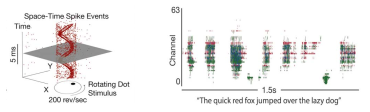
\includegraphics[width=0.8\textwidth]{neuro-sensors}
    \caption{Sample output of a silicon retina (left) and cochlea (right). Adapted from~\cite{liu2010neuromorphic}.}
    \label{fig:neuro:retina-cochlea}
  \end{center}
\end{figure}
Both sensors' output is transmitted using an address-event representation (AER). A sample of a retina and cochlea is presented in Figure~\ref{fig:neuro:retina-cochlea}.